\documentclass[11pt,a4paper]{report}

\usepackage[utf8]{inputenc}
\usepackage{titling}
\usepackage[german]{babel}
\usepackage[T1]{fontenc}
\usepackage{amsmath}
\usepackage{amsfonts}
\usepackage{amssymb}
\usepackage[left=3cm,right=2cm,top=2.5cm,bottom=2cm]{geometry}
\usepackage{graphicx}
\usepackage{fancyhdr}
\usepackage{color}
\usepackage[
colorlinks=true,
urlcolor=blue,
linkcolor=black
]{hyperref}
\pagestyle{fancy}

\lhead{Leon Kamuf}
\chead{ak18b}
\rhead{27.01.2019}

\lfoot{}
\cfoot{\thepage}
\rfoot{}

\renewcommand{\headrulewidth}{0.4pt}
\renewcommand{\footrulewidth}{0.4pt}

\begin{document}
	\begin{titlepage}
		
		\pretitle{
			\vskip -3em
			\begin{figure}[h]
				\begin{center}
					
\includegraphics[scale=0.55]{Logo.png}
				\end{center}
			\end{figure}
			\begin{center}
				\vskip -2em
				\large{Wintersemester 2018/19\\Softwaretechnikpraktikum} \vskip 9em
				\rule{5in}{0.4pt}\par \vskip 0.5em
			}
			\posttitle{\par\rule{5in}{0.4pt} \vskip 4em
				\Large Gruppe: ak18b \vskip 1.5em
				\normalsize Betreuer: Benjamin Lucas Friedland, Michael Fritz\vskip 1em
				\normalsize Gruppenmitglieder: Alexander Zwisler, Leon Kamuf, Leon Rudolph, Maurice Eisenblätter, Maximilian Gläfcke, Robin Seidel, Sina Opitz, Steve Woywod
		\end{center}}
		
		\title{\textbf{\Huge App zur Inventarisierung von Unternehmenswerten}\vskip 0.5em \huge Entwurfsbeschreibung}
		\date{}
		\maketitle
	\end{titlepage}
	\setcounter{secnumdepth}{4}
	\setcounter{tocdepth}{4}
	\tableofcontents
	\thispagestyle{empty}
	\newpage
	\setcounter{page}{1}
	\renewcommand\thesection{\arabic{section}}
	
	\section{Visionen und Ziele}
	Unser Ziel ist es, eine frei konfigurierbare Web-App für Google Chrome zur vollständigen Inventarisierung zu entwickeln und optimieren. Um eine optimierte Übersicht zu gewährleisten, kann das gesamte Inventar in Itemtypen gegliedert werden, die unterschiedliche Eigenschaften besitzen. Innerhalb der Itemtypen existiert auch eine vollständige Anzeige der einzelnen Items. Für alle Itemtypen können Felder, darunter Pflichtfelder, 'Unique'-Felder erstellt werden, um eine hohe Konfigurierbarkeit zu gewährleisten. Außerdem kann eingestellt werden, welche Felder in der Item-Auflistung und welche nur bei der Detailansicht angezeigt werden. Weiterhin gibt es eine Sortier- sowie Suchfunktion, um eine optimale Übersicht und schnelle Bedienung zu ermöglichen.\\
Damit auch alle Daten sicher bleiben, gibt es ein Account-System mit gesicherter Login- und Logout-Funktion. Der Admin kann außerdem Benutzergruppen erstellen und beliebig konfigurieren, um Rechte zu vergeben. So können nur bestimmte Nutzer beispielsweise Items bearbeiten oder löschen.\\
	Auch die Mehrsprachigkeit (Deutsch und Englisch) ist ein Ziel.
	
	\section{Rahmenbedingungen und Produktübersicht}
	Das Projekt basiert auf einem Server-Client-Grundkonzept mit einem Back-End und Front-End. Zur Speicherung der Daten wird eine MariaDB und als Schnittstelle zwischen Client und Server eine REST-Api verwendet.
	\subsection{Back-End}
	Das Back-End bildet die Schnittstelle zwischen der Datenbank (MariaDB) und dem Client.
	Es sorgt im Wesentlichen dafür, dass die vom Client übertragenen Daten vollständig und korrekt sind, sowie für das Erstellen, Manipulieren und Löschen der dynamischen Datensätze (Items).\\
	Der Server selbst versteht nur HTTP-Anfragen vom Content-Type 'applications/json' und antwortet auch in diesem.
	
	\subsection{Front-End}
	Das Front-End wird komplett in Angular entwickelt und dient als Benutzeroberfläche, auf der sich alle Funktionen der Web-App übersichtlich finden und genutzt werden. Es existiert außerdem eine REST-Api zwischen Back-End und Front-End.
	
	\section{Grundsätzliche Struktur- und Entwurfsprinzipien}
	\subsection{Programmiersprache}
	Das gesamte Projekt wird in \texttt{TypeScript} geschrieben. Das Front-End benutzt für den Style von \texttt{HTML CSS}, welches durch den \texttt{sass}-Precompiler generiert wird.
	
	\subsection{Vorgehensweise}
	Die Entwicklung findet zuallererst im Back-End statt, wo die Funktionalitäten implementiert und optimiert werden, bevor dazu ein passendes Front-End entwickelt wird. Anschließend wird beides über die REST-Api miteinander verbunden, getestet und ggf. angepasst. Der Style des Userinterfaces wird dann zum Schluss erstellt.
	\clearpage
	
	\subsection{Back-End}
	Alle Eingaben, die der Nutzer im Front-End tätigt, werden über die REST-Api ins Back-End übergeben, vom Server auf Korrektheit überprüft und anschließend in der Datenbank gespeichert. Des Weiteren existiert eine Serverstruktur, welche Daten (bei Sortier- und Suchanfragen) aus der Datenbank ausliest und an die anfragenden Clients weiterleitet.\\
	Auch die Datensicherung und die damit verbundene Rechteverwaltung wird im Back-End definiert und somit die Anzeige der Elemente im Front-End gesteuert.
	
	\subsection{Front-End}
	Die im Back-End definierte Rechteverwaltung steuert die Anzeige im Front-End. Während Benutzer, die alle Rechte besitzen, Buttons zum Ändern und Löschen angezeigt bekommen, fehlen diese bei anderen Benutzern (noch nicht implementiert). 
	Gästen wird dabei nur die Startseite und die Login-Seite angezeigt. 
	Auf der Login-Seite existiert ein Fenster, wo Username und Passwort abgefragt werden. 
	Die Eingabe im Passwort-Feld wird zum Schutz ausgeblendet.
	
	\begin{center}
		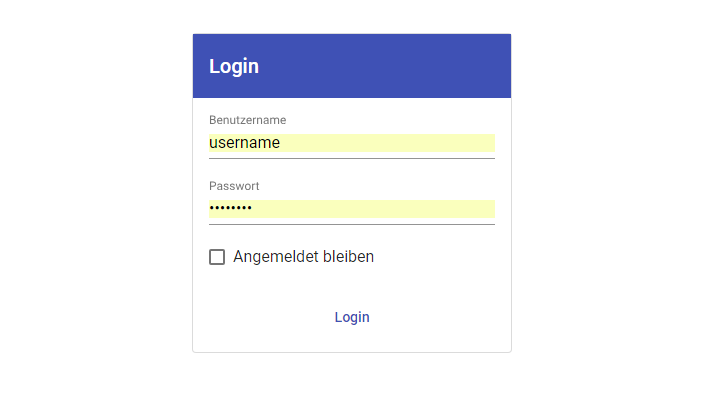
\includegraphics[scale=0.5]{login.png}\\
	\end{center}
	
	Allen eingeloggten Benutzern wird eine Übersicht der Objekttypen angezeigt. 
	Dort können auch neue Objekttypen erstellt und bereits vorhandene bearbeitet werden. 
	Bei den Einstellungen der Objekttypen werden die Eigenschaften der Items festgehalten. \\
	
	\begin{center}
		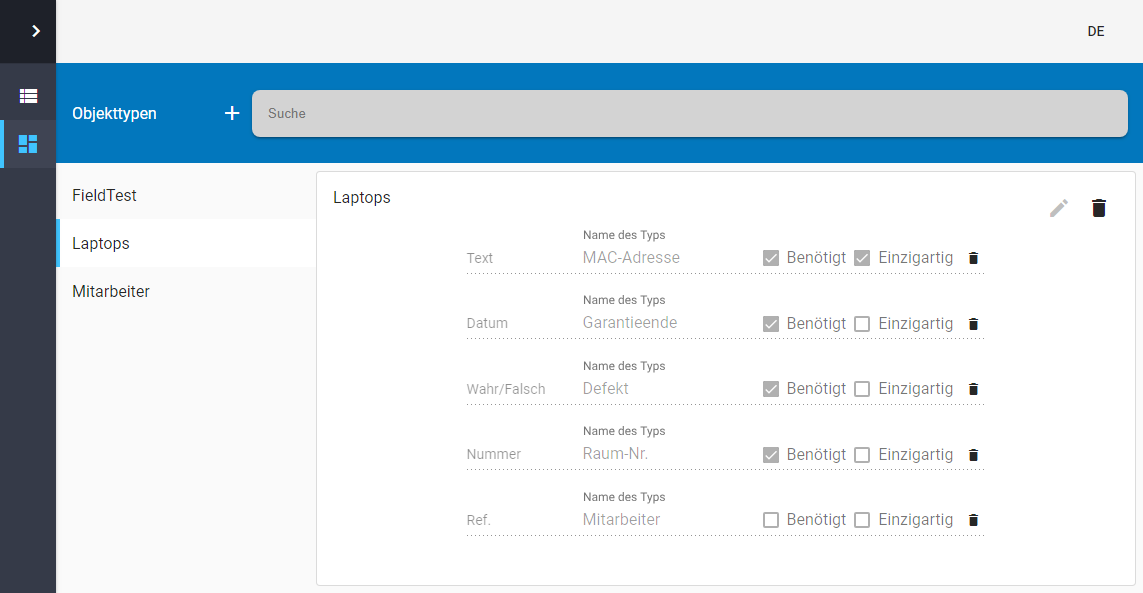
\includegraphics[scale=0.3]{itemtyp.png}
		\\Übersicht Objekttypen mit Einstellungen
	\end{center}
	
	\newpage
	
	Durch einen Button links im Menü gelangt man dann zu der Übersicht der einzelnen Items innerhalb eines Objekttyps.
	Über einen Tab links kann man zwischen den Objekttypen switchen.\\
		
	\begin{center}
		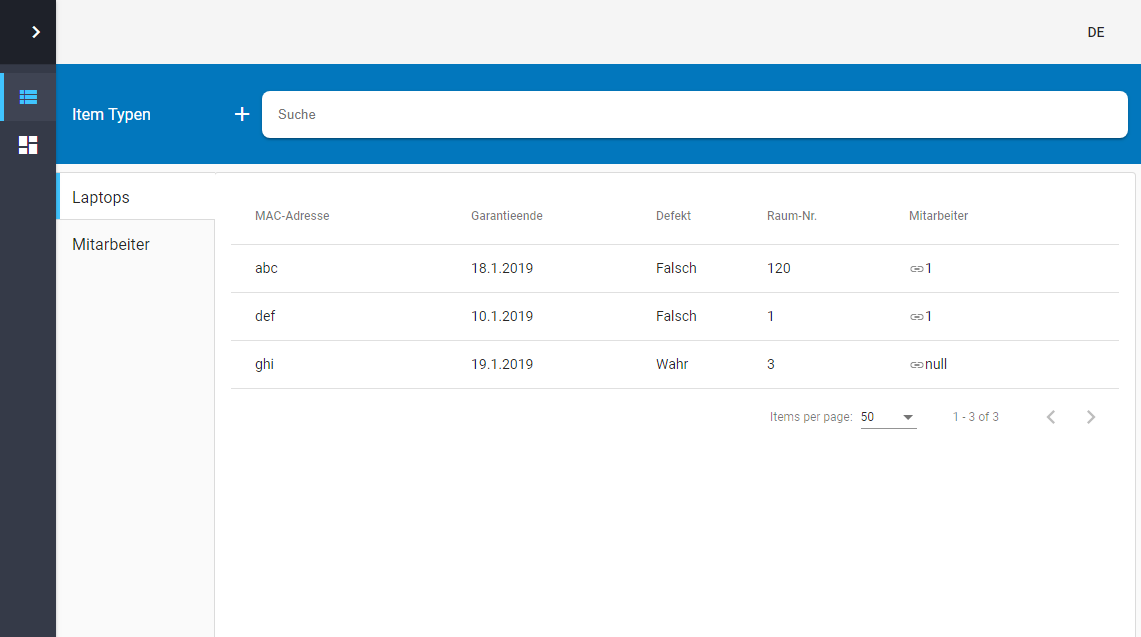
\includegraphics[scale=0.3]{uebersicht.png}\\
		Übersicht Items eines Typs\\
	\end{center}
	
	Dort können neue Items hinzugefügt, bearbeitet und gelöscht werden.\\
	
	\begin{center}
		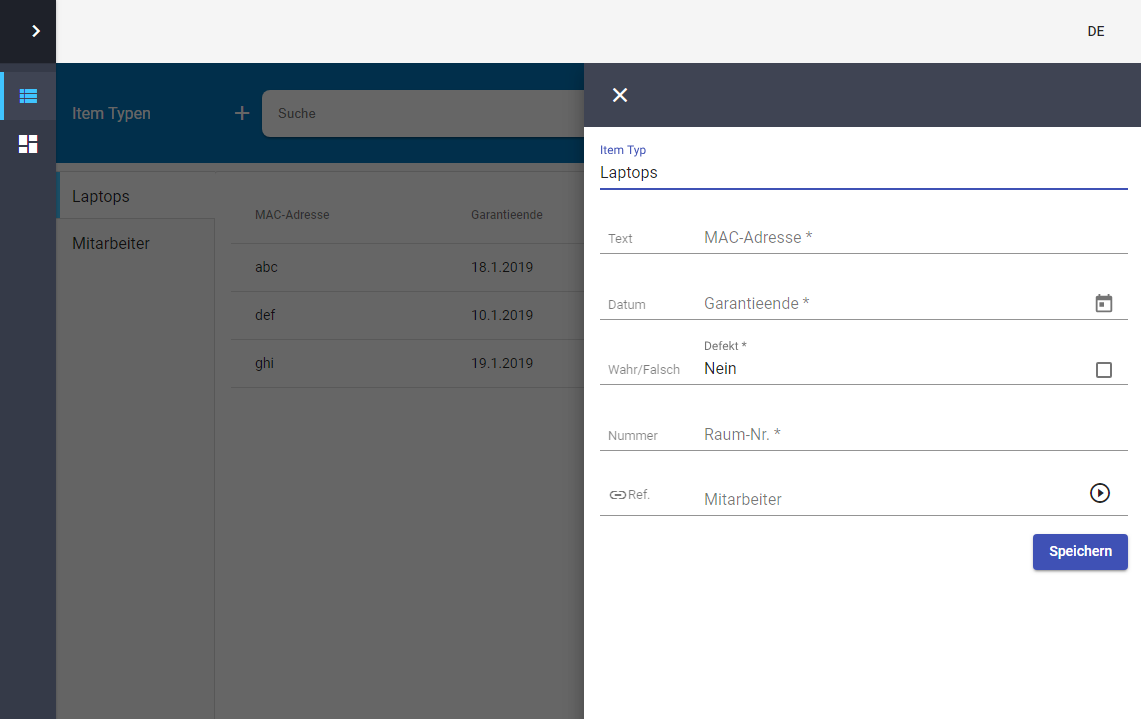
\includegraphics[scale=0.3]{eigenschaften.png}\\
	\end{center}
	
	Außerdem gelangt man über den Button links oben zum Sprachwechsler und zum Logout.
	Je nach Benutzergruppe werden Buttons und die damit verbundenen Funktionen ausgeblendet.
	So sehen nicht alle den Button, um Items zu löschen oder Itemtypen zu erstellen.
	
	\section{Struktur- und Entwurfprinzipien einzelner Pakete}
	Das Projekt besitzt zwei Pakete, den \texttt{client} und den \texttt{server}. 
	Innerhalb des Projekt-Pakets, befinden sich außerdem alle Packages, die benötigt werden, und die REST-Api als Schnittstelle zwischen dem Client und Server. 
	In jedem Paket befinden sich die Auflistung der benutzten Frameworks und Tools, ein Text-Paket mit Testdaten und die \texttt{src}-Pakete, wo die Funktionalitäten festgehalten werden.
	
	\subsection{server}
	Im \texttt{server}-Paket wird der HTTP-Server initialisiert, die einzelnen Seiten (ggf. mit Sichtbarkeitseinschränkungen) geladen und die Verbindung zur Datenbank hergestellt.
	
	\subsubsection*{\texttt{/types}}
	Hier werden für TypeScript fehlende Typen, wie zum Beispiel 'MariaDB' erfasst und niedergeschrieben.
	
	\subsubsection*{\texttt{/src/app.ts}}
	Ist der Core des Back-Ends und initialisiert die Datenbank und den Express-Server.
	
	\subsubsection*{\texttt{/src/index.ts}}
	Hier wird die Config eingelesen und der HTTP(S)-Server, sowie die App (/src/app.ts) gestartet.

	\subsubsection*{\texttt{/src/api}}
	Hier werden alle Endpunkte der API definiert, sowie der Funktion implementiert.
	
	\subsubsection*{\texttt{/src/database}}
	Hier werden alle Datenbank-Abfragen definiert und implementiert, außerdem gibt es Modellklassen für die Datenbank.
	
	\subsubsection*{\texttt{/src/types.ts}}
	\textbf{War schon beim letzten Release dabei aber nicht aufgelistet. Unwichtig???}
	
	
	\subsection{client}
	
	\subsubsection*{\texttt{/src/assets}}
	Hier werden die Sprachen für den Sprachregler definiert.	
		
	\subsubsection*{\texttt{/src/app}}
	Hier befinden sich die einzelnen Komponenten, aus welchen sich die Web-App zusammensetzt.

	\subsubsection*{\texttt{/src/app/company}}
	Hier befinden sich alle nötigen Komponenten und Funktion, um die Unternehmensverwaltung zu realisieren. 

	\subsubsection*{\texttt{/src/app/items}}
	Hier werden alle Komponenten der Seite, die mit den Items zu tun haben, und die dazugehörigen Funktionen definiert und initialisiert. 
	Dies beinhaltet unter anderem das Anzeigen von Items, im Bezug auf dessen Typen, und die Suchleiste.
	
	\subsubsection*{\texttt{/src/app/models}}
	Hier werden alle benötigten Interfaces erzeugt, welche dann in Komponente importiert werden können, sollten sie gebraucht werden.
	
	\subsubsection*{\texttt{/src/app/roles}}
	\textbf{Unwichtig, da noch nicht implementiert?}
	
	\subsubsection*{\texttt{/src/app/shared}}
	\textbf{Unwichtig, da noch nicht implementiert?}
	
	\subsubsection*{\texttt{/src/app/types}}
	Hier werden alle Komponenten der Seite, welche mit Itemtypen zu tun haben, und die dazugehörigen Funktionen definiert und initialisiert.
	Dazugehörig ist, zum Beispiel 'Globale Pflichtfelder' und das Anzeigen von Itemtypen.
	
	\subsubsection*{\texttt{/src/app/user}}
	Hier werden alle Komponenten, zur Darstellung von Benutzern, und die entsprechenden Funktionen definiert und initialisiert.
	
	\subsubsection*{\texttt{/src/app/shell}}
	Hier wird das grobe Userinterface definiert. Dazu gehören die Authentifizierung, Sprachselektor, Navigation und das Login-Fenster.
	
	\subsubsection*{\texttt{/src/environments}}
	Hier befinden sich die Einstellungen für die verschiedenen Umgebungen, in denen die Applikation laufen soll.
	
	\section{Datenmodell}
	Die Datenbank muss sehr dynamisch sein, da die einzelnen Daten, die gespeichert werden sollen, frei konfigurierbar sind.\\
	Bei den Itemtypen werden die einzelnen Eigenschaften, die jedes Item des Typs besitzen soll, definiert. 
	Es muss dabei ein \texttt{key} gesetzt werden, um den Datensatz eindeutig zu bestimmen. 
	Diesen Key setzt der Benutzer. 
	Außerdem legt der Benutzer selbst fest, welche Felder Pflichtfelder sind.\\
	Die Items innerhalb des Typs werden anhand der Einstellungen des Itemtyps festgestellt. 
	Bei jedem Hinzufügen und Ändern eines Items wird darauf geachtet, dass ein eindeutiger Key gesetzt und alle Pflichtfelder erfüllt wurden. 
	Erst dann speichert der Server die eingegeben Daten in die Datenbank.\\
	
	\newpage	
	
	\section{Glossar}
	
	\subsection*{Web-App}
	Eine Webanwendung (auch Webapplikation, kurz Web-App) ist eine Anwendung nach dem Server-Client-Prinzip. 
	Der große Unterschied zu den klassischen Desktop-Apps besteht darin, dass die Anwendung nicht lokal auf dem Computer, sondern auf einem Webserver online ausgeführt wird.
	
	\subsection*{Server-Client-Prinzip}
	Das Client-Server-Prinzip beschreibt eine Möglichkeit, innerhalb eines Netzwerks zu kommunizieren. 
	Der sogenannte Client, kann dabei Dienste und Daten vom Server abfragen, die dann vom Server bearbeitet und an den Client zurück übermittelt werden.
	
	\subsection*{Back-End / Front-End}
	Viele Vorgänge und Anwendungen lassen sich in Front- und Back-End unterteilen. 
	Front-End ist hierbei das Userinterface, welches der Benutzer sieht.\\
	Im Back-End hingegen befinden sich die Prozesse, die im Hintergrund ausgeführt werden und die Benutzung der Anwendung ermöglicht.\\
	In unserem Fall ist der Server das Back-End und der Client das Front-End.
	
	\subsection*{MariaDB}
	MariaDB ist eine freies Datenbankmanagementsystem, welches durch eine Abspaltung aus MySQL entstanden ist.
	
	\subsection*{REST-Api}
	Die \textbf{Re}presentational \textbf{S}tate \textbf{T}ransfer des \textbf{A}pplication \textbf{P}rogramming \textbf{I}nterfaces ist eine Programmierschnittstelle zwischen Server und Client.
	
	\subsection*{TypeScript}
	TypeScript ist eine Scriptsprache, die von jedem Browser und Betriebssystem unterstützt wird. 
	Sie ist eine Erweiterung von Javascript.

\end{document}